% Options for packages loaded elsewhere
\PassOptionsToPackage{unicode}{hyperref}
\PassOptionsToPackage{hyphens}{url}
%
\documentclass[
]{book}
\usepackage{amsmath,amssymb}
\usepackage{lmodern}
\usepackage{iftex}
\ifPDFTeX
  \usepackage[T1]{fontenc}
  \usepackage[utf8]{inputenc}
  \usepackage{textcomp} % provide euro and other symbols
\else % if luatex or xetex
  \usepackage{unicode-math}
  \defaultfontfeatures{Scale=MatchLowercase}
  \defaultfontfeatures[\rmfamily]{Ligatures=TeX,Scale=1}
\fi
% Use upquote if available, for straight quotes in verbatim environments
\IfFileExists{upquote.sty}{\usepackage{upquote}}{}
\IfFileExists{microtype.sty}{% use microtype if available
  \usepackage[]{microtype}
  \UseMicrotypeSet[protrusion]{basicmath} % disable protrusion for tt fonts
}{}
\makeatletter
\@ifundefined{KOMAClassName}{% if non-KOMA class
  \IfFileExists{parskip.sty}{%
    \usepackage{parskip}
  }{% else
    \setlength{\parindent}{0pt}
    \setlength{\parskip}{6pt plus 2pt minus 1pt}}
}{% if KOMA class
  \KOMAoptions{parskip=half}}
\makeatother
\usepackage{xcolor}
\IfFileExists{xurl.sty}{\usepackage{xurl}}{} % add URL line breaks if available
\IfFileExists{bookmark.sty}{\usepackage{bookmark}}{\usepackage{hyperref}}
\hypersetup{
  pdftitle={Panel Analyses Report},
  pdfauthor={David BYAMUNGU},
  hidelinks,
  pdfcreator={LaTeX via pandoc}}
\urlstyle{same} % disable monospaced font for URLs
\usepackage{color}
\usepackage{fancyvrb}
\newcommand{\VerbBar}{|}
\newcommand{\VERB}{\Verb[commandchars=\\\{\}]}
\DefineVerbatimEnvironment{Highlighting}{Verbatim}{commandchars=\\\{\}}
% Add ',fontsize=\small' for more characters per line
\usepackage{framed}
\definecolor{shadecolor}{RGB}{248,248,248}
\newenvironment{Shaded}{\begin{snugshade}}{\end{snugshade}}
\newcommand{\AlertTok}[1]{\textcolor[rgb]{0.94,0.16,0.16}{#1}}
\newcommand{\AnnotationTok}[1]{\textcolor[rgb]{0.56,0.35,0.01}{\textbf{\textit{#1}}}}
\newcommand{\AttributeTok}[1]{\textcolor[rgb]{0.77,0.63,0.00}{#1}}
\newcommand{\BaseNTok}[1]{\textcolor[rgb]{0.00,0.00,0.81}{#1}}
\newcommand{\BuiltInTok}[1]{#1}
\newcommand{\CharTok}[1]{\textcolor[rgb]{0.31,0.60,0.02}{#1}}
\newcommand{\CommentTok}[1]{\textcolor[rgb]{0.56,0.35,0.01}{\textit{#1}}}
\newcommand{\CommentVarTok}[1]{\textcolor[rgb]{0.56,0.35,0.01}{\textbf{\textit{#1}}}}
\newcommand{\ConstantTok}[1]{\textcolor[rgb]{0.00,0.00,0.00}{#1}}
\newcommand{\ControlFlowTok}[1]{\textcolor[rgb]{0.13,0.29,0.53}{\textbf{#1}}}
\newcommand{\DataTypeTok}[1]{\textcolor[rgb]{0.13,0.29,0.53}{#1}}
\newcommand{\DecValTok}[1]{\textcolor[rgb]{0.00,0.00,0.81}{#1}}
\newcommand{\DocumentationTok}[1]{\textcolor[rgb]{0.56,0.35,0.01}{\textbf{\textit{#1}}}}
\newcommand{\ErrorTok}[1]{\textcolor[rgb]{0.64,0.00,0.00}{\textbf{#1}}}
\newcommand{\ExtensionTok}[1]{#1}
\newcommand{\FloatTok}[1]{\textcolor[rgb]{0.00,0.00,0.81}{#1}}
\newcommand{\FunctionTok}[1]{\textcolor[rgb]{0.00,0.00,0.00}{#1}}
\newcommand{\ImportTok}[1]{#1}
\newcommand{\InformationTok}[1]{\textcolor[rgb]{0.56,0.35,0.01}{\textbf{\textit{#1}}}}
\newcommand{\KeywordTok}[1]{\textcolor[rgb]{0.13,0.29,0.53}{\textbf{#1}}}
\newcommand{\NormalTok}[1]{#1}
\newcommand{\OperatorTok}[1]{\textcolor[rgb]{0.81,0.36,0.00}{\textbf{#1}}}
\newcommand{\OtherTok}[1]{\textcolor[rgb]{0.56,0.35,0.01}{#1}}
\newcommand{\PreprocessorTok}[1]{\textcolor[rgb]{0.56,0.35,0.01}{\textit{#1}}}
\newcommand{\RegionMarkerTok}[1]{#1}
\newcommand{\SpecialCharTok}[1]{\textcolor[rgb]{0.00,0.00,0.00}{#1}}
\newcommand{\SpecialStringTok}[1]{\textcolor[rgb]{0.31,0.60,0.02}{#1}}
\newcommand{\StringTok}[1]{\textcolor[rgb]{0.31,0.60,0.02}{#1}}
\newcommand{\VariableTok}[1]{\textcolor[rgb]{0.00,0.00,0.00}{#1}}
\newcommand{\VerbatimStringTok}[1]{\textcolor[rgb]{0.31,0.60,0.02}{#1}}
\newcommand{\WarningTok}[1]{\textcolor[rgb]{0.56,0.35,0.01}{\textbf{\textit{#1}}}}
\usepackage{longtable,booktabs,array}
\usepackage{calc} % for calculating minipage widths
% Correct order of tables after \paragraph or \subparagraph
\usepackage{etoolbox}
\makeatletter
\patchcmd\longtable{\par}{\if@noskipsec\mbox{}\fi\par}{}{}
\makeatother
% Allow footnotes in longtable head/foot
\IfFileExists{footnotehyper.sty}{\usepackage{footnotehyper}}{\usepackage{footnote}}
\makesavenoteenv{longtable}
\usepackage{graphicx}
\makeatletter
\def\maxwidth{\ifdim\Gin@nat@width>\linewidth\linewidth\else\Gin@nat@width\fi}
\def\maxheight{\ifdim\Gin@nat@height>\textheight\textheight\else\Gin@nat@height\fi}
\makeatother
% Scale images if necessary, so that they will not overflow the page
% margins by default, and it is still possible to overwrite the defaults
% using explicit options in \includegraphics[width, height, ...]{}
\setkeys{Gin}{width=\maxwidth,height=\maxheight,keepaspectratio}
% Set default figure placement to htbp
\makeatletter
\def\fps@figure{htbp}
\makeatother
\setlength{\emergencystretch}{3em} % prevent overfull lines
\providecommand{\tightlist}{%
  \setlength{\itemsep}{0pt}\setlength{\parskip}{0pt}}
\setcounter{secnumdepth}{5}
\usepackage{booktabs}
\usepackage{booktabs}
\usepackage{longtable}
\usepackage{array}
\usepackage{multirow}
\usepackage{wrapfig}
\usepackage{float}
\usepackage{colortbl}
\usepackage{pdflscape}
\usepackage{tabu}
\usepackage{threeparttable}
\usepackage{threeparttablex}
\usepackage[normalem]{ulem}
\usepackage{makecell}
\usepackage{xcolor}
\ifLuaTeX
  \usepackage{selnolig}  % disable illegal ligatures
\fi
\usepackage[]{natbib}
\bibliographystyle{apalike}

\title{Panel Analyses Report}
\author{David BYAMUNGU}
\date{2021-06-16}

\begin{document}
\maketitle

{
\setcounter{tocdepth}{1}
\tableofcontents
}
\hypertarget{prerequis}{%
\chapter{Prerequis}\label{prerequis}}

Ceci est \emph{une étude} des données de panel avec \textbf{Markdown}.

The \textbf{bookdown} package can be installed from CRAN or Github:

La structure de ce rapport est que chaque fichier RMD porte un chapitre et un thème bien spécifique de notre analyse

Nous avions utilisé XeLaTeX pour compiler ce document en PDF.

\hypertarget{intro}{%
\chapter{Introduction}\label{intro}}

You can label chapter and section titles using \texttt{\{\#label\}} after them, e.g., we can reference Chapter \ref{intro}. If you do not manually label them, there will be automatic labels anyway, e.g., Chapter \ref{methods}.

Figures and tables with captions will be placed in \texttt{figure} and \texttt{table} environments, respectively.

\begin{Shaded}
\begin{Highlighting}[]
\FunctionTok{par}\NormalTok{(}\AttributeTok{mar =} \FunctionTok{c}\NormalTok{(}\DecValTok{4}\NormalTok{, }\DecValTok{4}\NormalTok{, .}\DecValTok{1}\NormalTok{, .}\DecValTok{1}\NormalTok{))}
\FunctionTok{plot}\NormalTok{(pressure, }\AttributeTok{type =} \StringTok{\textquotesingle{}b\textquotesingle{}}\NormalTok{, }\AttributeTok{pch =} \DecValTok{19}\NormalTok{)}
\end{Highlighting}
\end{Shaded}

\begin{figure}

{\centering 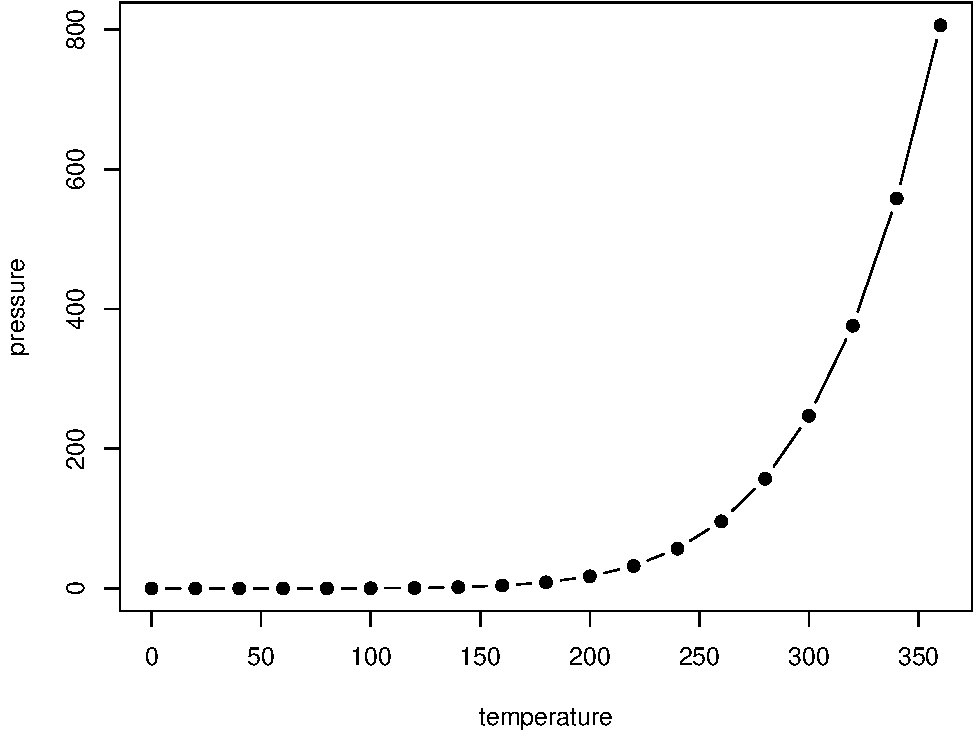
\includegraphics[width=0.8\linewidth]{panel-analyses-book_files/figure-latex/nice-fig-1} 

}

\caption{Here is a nice figure!}\label{fig:nice-fig}
\end{figure}

Reference a figure by its code chunk label with the \texttt{fig:} prefix, e.g., see Figure \ref{fig:nice-fig}. Similarly, you can reference tables generated from \texttt{knitr::kable()}, e.g., see Table \ref{tab:nice-tab}.

\begin{Shaded}
\begin{Highlighting}[]
\NormalTok{knitr}\SpecialCharTok{::}\FunctionTok{kable}\NormalTok{(}
  \FunctionTok{head}\NormalTok{(iris, }\DecValTok{20}\NormalTok{), }\AttributeTok{caption =} \StringTok{\textquotesingle{}Here is a nice table!\textquotesingle{}}\NormalTok{,}
  \AttributeTok{booktabs =} \ConstantTok{TRUE}
\NormalTok{)}
\end{Highlighting}
\end{Shaded}

\begin{table}

\caption{\label{tab:nice-tab}Here is a nice table!}
\centering
\begin{tabular}[t]{rrrrl}
\toprule
Sepal.Length & Sepal.Width & Petal.Length & Petal.Width & Species\\
\midrule
5.1 & 3.5 & 1.4 & 0.2 & setosa\\
4.9 & 3.0 & 1.4 & 0.2 & setosa\\
4.7 & 3.2 & 1.3 & 0.2 & setosa\\
4.6 & 3.1 & 1.5 & 0.2 & setosa\\
5.0 & 3.6 & 1.4 & 0.2 & setosa\\
\addlinespace
5.4 & 3.9 & 1.7 & 0.4 & setosa\\
4.6 & 3.4 & 1.4 & 0.3 & setosa\\
5.0 & 3.4 & 1.5 & 0.2 & setosa\\
4.4 & 2.9 & 1.4 & 0.2 & setosa\\
4.9 & 3.1 & 1.5 & 0.1 & setosa\\
\addlinespace
5.4 & 3.7 & 1.5 & 0.2 & setosa\\
4.8 & 3.4 & 1.6 & 0.2 & setosa\\
4.8 & 3.0 & 1.4 & 0.1 & setosa\\
4.3 & 3.0 & 1.1 & 0.1 & setosa\\
5.8 & 4.0 & 1.2 & 0.2 & setosa\\
\addlinespace
5.7 & 4.4 & 1.5 & 0.4 & setosa\\
5.4 & 3.9 & 1.3 & 0.4 & setosa\\
5.1 & 3.5 & 1.4 & 0.3 & setosa\\
5.7 & 3.8 & 1.7 & 0.3 & setosa\\
5.1 & 3.8 & 1.5 & 0.3 & setosa\\
\bottomrule
\end{tabular}
\end{table}

You can write citations, too. For example, we are using the \textbf{bookdown} package \citep{R-bookdown} in this sample book, which was built on top of R Markdown and \textbf{knitr} \citep{xie2015}.

\hypertarget{literature}{%
\chapter{Literature}\label{literature}}

\hypertarget{the-one-way-error-component-regression-model}{%
\chapter{The One-way Error Component Regression Model}\label{the-one-way-error-component-regression-model}}

\hypertarget{introduction}{%
\section{INTRODUCTION}\label{introduction}}

A panel data regression differs from a regular time-series or cross-section regression in that it
has a double subscript on its variables, i.e.

\[  y_{it}= \alpha + X_{it}^{'} \beta + u_{it}                      \]
\[ i=1, ... , N  ; t=1, ... ,T  \]
(2.1)

with \[ i \] denoting households, individuals, firms, countries, etc. and t denoting time. The i subscript, therefore, denotes the cross-section dimension whereas t denotes the time-series dimension. \[ \alpha  \] is a scalar, \[ \beta \] is \[ K × 1 \] and Xi t is the \[ it_{th} \] observation on K explanatory variables.
Most of the panel data applications utilize a one-way error component model for the disturbances, with

\[ u_{it}= \mu_i +  v_{it}      \]
(2.2)

where μi denotes the unobservable individual-specific effect and νi t denotes the remainder disturbance. For example, in an earnings equation in labor economics, yi t will measure earnings of the head of the household, whereas \[ X_{it} \] may contain a set of variables like experience, education, union membership, sex, race, etc. Note that μi is time-invariant and it accounts for any individual-specific effect that is not included in the regression. In this case we could think of it as the individual's unobserved ability. The remainder disturbance \[ v_{it} \] varies with individuals and time and can be thought of as the usual disturbance in the regression. Alternatively, for a production function utilizing data on firms across time, \[ y_{it} \] will measure output and \[ X_{it} \] will measure inputs. The unobservable firm-specific effects will be captured by the \[ \mu_i \]
and we can think of these as the unobservable entrepreneurial or managerial skills of the firm's executives. Early applications of error components in economics include Kuh (1959) on investment, Mundlak (1961) and Hoch (1962) on production functions and Balestra and Nerlove (1966) on demand for natural gas. In vector form (2.1) can be written as

\[ y= \alpha i_{NT} + X \beta + u = Z \delta + u      \] (2.3)

\[ y= \alpha i_{NT} + X \beta + u = Z \delta + u      \] (2.3)

where \[ y \] is \[ NT × 1 \], \[ X \] is \[ NT × K \], \[ Z = [ι_{NT} , X] \],
\[ \delta^{'} = (α^{'},\beta^{'}) \] and \[ι_NT\] is a vector of ones of
dimension NT. Also, (2.2) can be written as

\[ u=Z_\mu \mu +v  \] (2.4)

\[  y_{it} = \alpha + X_{it}^{'} + U_{it}   \] , \$ i=1,\ldots,N ; t=1,\ldots,T \$
with i denoting households, individuals, firms, countries, etc. and t denoting time. The i subscript, therefore, denotes the cross-section dimension whereas t denotes the time-series dimension. \$ \alpha \$ is a scalar, \$ \beta \$ is \$ K × 1 \$ and \$X\_\{it\} \$is the \$ it\^{}\{th\} \$ observation on K explanatory variables.
disturbances, with it
\[ u_{it}=u_i  + v_{it}     \]

where μi denotes the unobservable individual-specific effect and \(ν{it}\) denotes the remainder disturbance. For example, in an earnings equation in labor economics, \(y_{it}\) will measure earnings of the head of the household, whereas Xi t may contain a set of variables like experience, education, union membership, sex, race, etc. Note that μi is time-invariant and it accounts for any individual-specific effect that is not included in the regression. In this case we could think of it as the individual's unobserved ability. The remainder disturbance \$ ν\{it\} \$ varies with individuals
and time and can be thought of as the usual disturbance in the regression. Alternatively, for a production function utilizing data on firms across time, \$ y\_\{it\} \$ will measure output and \$ X\_\{it\} \$ will measure inputs. The unobservable firm-specific effects will be captured by the \$ \mu\_i \$ and we can think of these as the unobservable entrepreneurial or managerial skills of the firm's executives. Early applications of error components in economics include Kuh (1959) on investment, Mundlak (1961) and Hoch (1962) on production functions and Balestra and Nerlove (1966) on demand for natural gas. In vector form (2.1) can be written as

\[ y= \alpha i_{NT}  + X\beta +u = Z\delta + u \]

where \(y\) is \$ NT × 1\$ , X is \(NT × K\) , \$ Z = {[}i\_\{NT\} , X{]} \$ , \$ \delta\^{}\{`\}=(\alpha\textsuperscript{\{'\},\beta}\{'\}) \$ and \(i_{NT}\) is a vector of ones of dimension \(NT\) . Also, (2.2) can be written as

\[ u=Z_\mu \mu  + v\]
(2.4)

where \$ u\^{}\{`\} = (u\_\{11\}, . . . , u\_\{1T\} , u\_\{21\}, . . . , u\_\{2T\}, . . . , u\_\{N1\}, . . . , u\_\{NT\} ) \$ with the observations stacked
such that the slower index is over individuals and the faster index is over time.\$ Z\_\mu = IN \otimes ιT \$
where IN is an identity matrix of dimension N, ιT is a vector of ones of dimension T and \$ \otimes \$ denotes Kronecker product. \$ Z\_\mu \$ is a selector matrix of ones and zeros, or simply the matrix of individual dummies that one may include in the regression to estimate theμi if they are assumed to
be fixed parameters. \$ \mu\^{}\{'\} = (\mu\_1, . . . , \mu\_N )\$ and \(ν^{'} = (ν11, . . . , ν_{1T} , . . . , ν_{N1}, . . . , ν_{NT} )\). Note that

\hypertarget{methods}{%
\chapter{Methods}\label{methods}}

We describe our methods in this chapter.

Les données de panel, ou données longitudinales possèdent les deux dimensions précédentes (individuelle et temporelle). En effet, il est souvent intéressant d'identifier l'effet associé à chaque individu (un effet qui ne varie pas dans le temps, mais qui varie d'un individu à un autre). Cet effet peut être fixe ou aléatoire.

Par conséquent, le modèle en données de panel s'écrit comme un modèle à double indice qui prend la forme suivante :

\[ Y_{it}= \alpha_i\sum_{k}\beta_{ki}x_{ki}+ \epsilon_{it} \]

avec
\[ i:1 \rightarrow N \]\\
et
\[ t:1 \rightarrow T \]

La double dimension qu'offrent les données de panel est un atout majeur. En effet, si les données en séries temporelles permettent d'étudier l'évolution des relations dans le temps, elles ne permettent pas de contrôler l'hétérogénéité entre les individus. A l'inverse, les données en coupes transversales permettent d'analyser l'hétérogénéité entre les individus mais elles ne peuvent pas tenir compte des comportements dynamiques, puisque la dimension temporelle est exclue du champ d'analyse.

Ainsi, en utilisant des données de panel, on pourra exploiter les deux sources de variation de l'information statistique :
- Temporelle où variabilité intra-individuelle (within)
- et individuelle ou variabilité inter-individuelle (Between).

\hypertarget{analyses}{%
\chapter{Analyses}\label{analyses}}

Nous faisons \emph{application} des méthodes présentées dans le chapitre précédant pour l'analyse des données de pannel

Avant de passefr à la modélisation, nous ferons une description de nos variables d'interet d'une manière statique : nos prédicteurs et la variables réponses

\hypertarget{netoyage-de-la-base-des-donnuxe9es}{%
\section{Netoyage de la base des données}\label{netoyage-de-la-base-des-donnuxe9es}}

Apperçue globale des données

\begin{table}

\caption{\label{tab:unnamed-chunk-2}Echantillon de la base des données}
\centering
\begin{tabular}[t]{r|l|r|l|r|r}
\hline
N° & Country/destination & Year & Goods & Weight & Taxe\\
\hline
1 & AFRIQUE DU SUD & 2011 & GRUES SUR PNEUMATIQUE & 13500 & 0\\
\hline
2 & AFRIQUE DU SUD & 2011 & CAMION FAMIL & 12000 & 0\\
\hline
3 & AFRIQUE DU SUD & 2011 & CAMION SOMUL & 24000 & 0\\
\hline
4 & AFRIQUE DU SUD & 2013 & Café vert arabica k4 & 183 & 0\\
\hline
5 & AFRIQUE DU SUD & 2013 & Café vert arabica k4 & 19520 & 264771\\
\hline
6 & AFRIQUE DU SUD & 2013 & Café vert arabica k4 & 19520 & 272817\\
\hline
7 & AFRIQUE DU SUD & 2013 & Café vert arabica k4 & 19520 & 283220\\
\hline
8 & AFRIQUE DU SUD & 2013 & Café vert arabica k4 & 19520 & 264142\\
\hline
9 & AFRIQUE DU SUD & 2013 & CAMION & 24000 & 0\\
\hline
10 & AFRIQUE DU SUD & 2017 & Instruments et appareils du n°90.15 & 654 & 0\\
\hline
\end{tabular}
\end{table}

Voici la structure de la base des données

\begin{verbatim}
## Rows: 3,310
## Columns: 6
## $ `N°`                  <dbl> 1, 2, 3, 4, 5, 6, 7, 8, 9, 10, 11, 12, 13, 14, 1~
## $ `Country/destination` <chr> "AFRIQUE DU SUD", "AFRIQUE DU SUD", "AFRIQUE DU ~
## $ Year                  <dbl> 2011, 2011, 2011, 2013, 2013, 2013, 2013, 2013, ~
## $ Goods                 <fct> "GRUES SUR PNEUMATIQUE", "CAMION FAMIL", "CAMION~
## $ Weight                <dbl> 13500, 12000, 24000, 183, 19520, 19520, 19520, 1~
## $ Taxe                  <dbl> 0, 0, 0, 0, 264771, 272817, 283220, 264142, 0, 0~
\end{verbatim}

Voici les modalités de la variabme \texttt{Goods} qui signifie
\texttt{Marchandises}

\begin{table}

\caption{\label{tab:g}Modalités de la variable Goods à l'importation des donnees}
\centering
\begin{tabular}[t]{l}
\hline
x\\
\hline
0\\
\hline
3Café vert arabica, en feve K3\\
\hline
Abats comestibles,congeles,de chevaux,anes,mulets,ovins ou caprins\\
\hline
ABATS COMESTIBLES;CONGELES;DE CHEVAUX;ANES;MULETS;OVINS\\
\hline
Accessoires de radio diffusion\\
\hline
Accessoires de vehicules\\
\hline
Accumulateurs electriques\\
\hline
Acide acetique\\
\hline
ages de 5 ans ou moins\\
\hline
ages de plus de 5 ans\\
\hline
Agés de plus de 5 ans ou moins\\
\hline
Alcaloides du quinquina et leurs derives;\\
\hline
ALCOOL ETYLIQUE NON DENATURE\\
\hline
ambulance d'une cylindree excedant 2500 cm3\\
\hline
Antennes\\
\hline
Antennes et reflecteurs d'antennes\\
\hline
antennes et refleteurs\\
\hline
Appareils d'eclairage electriques\\
\hline
Appareils d'eclairage non electriques\\
\hline
Appareils d'eclairages electriques\\
\hline
Appareils du n°84.14\\
\hline
Appareils electrothermiques pour la\\
\hline
appareils pour la reception,la conversion et la transmission\\
\hline
Art et materiel d'athletisme\\
\hline
Articles confectionnes en textiles\\
\hline
Articles d'economie domestique,en\\
\hline
Articles de bureau\\
\hline
ARTICLES DE BUREAU\\
\hline
Articles de bureau ou de la papeterie\\
\hline
Articles de friperie\\
\hline
ARTICLES DE FRIPERIE\\
\hline
Articles et materiel d'athletisme\\
\hline
Ashok Layland\\
\hline
ASPIRATEUR ET ACCESSOIRES\\
\hline
Autes bois sciés\\
\hline
AUTRE MACHINE ET APPAREIL A IMPRIMER\\
\hline
AUTRE MINERAIS DE TITANE (Coltant)\\
\hline
AUTRE PARTIE DE PLANTE\\
\hline
AUTRE PEAUX\\
\hline
AUTRE PREP ALIMENTAIRE\\
\hline
Autre vehicules automobiles a usages speciaux\\
\hline
Autres\\
\hline
AUTRES\\
\hline
Autres  bois scies\\
\hline
Autres abats comestibles frais ou refrigérés de chevaux,anes,mulets,ovins,caprins\\
\hline
Autres abats comestibles,congeles,de chevaux,anes,mulets,ovins ou caprins\\
\hline
Autres accessoires de tuyauterie en fonte\\
\hline
Autres accumulateurs electriques\\
\hline
Autres appareils elevateurs, a action continue pour marchandises\\
\hline
Autres armes\\
\hline
Autres art de bureau ou de papeterie en papier\\
\hline
Autres Art de menage\\
\hline
Autres articles d'economie domestique, en\\
\hline
autres articles de bureau\\
\hline
AUTRES ARTICLES DE BUREAU OU D PAPETERIE EN PAPIER OU CARTON\\
\hline
Autres articles de bureau ou de papeterie en\\
\hline
Autres articles de campement\\
\hline
Autres articles de friperie\\
\hline
Autres articles de menage ou d'économie en aluminium\\
\hline
Autres articles de transport ou d'emballage\\
\hline
Autres articles en toles emailles\\
\hline
Autres babeurre,lait et creme\\
\hline
Autres babeurre,lait et creme caillés,yoghourt\\
\hline
autres baies fraiches\\
\hline
Autres bois\\
\hline
Autres bois plaques ou stratifies\\
\hline
AUTRES BOIS ROPICAUX SCIES LONG\\
\hline
Autres bois sciées\\
\hline
Autres bois scies\\
\hline
AUTRES BOIS SCIES\\
\hline
autres bois sciés\\
\hline
Autres bois sciés\\
\hline
Autres bois tropicaux, a scies long, sciages d'1 avives d'1 epaisseur superieure a 50mm\\
\hline
Autres bois tropicaux, scies lon, sciages avives d'1 epaisseur superieure a 50mm\\
\hline
Autres bois tropicaux,scies long\\
\hline
AUTRES BOIS TROPICAUX,SCIES LONG-SCIAGES AVIVESD'1 EPAISSEEUR SUPERIEURE A 50MM\\
\hline
Autres bois tropicaux,scies long,sciages avivées\\
\hline
Autres bois tropicaux,scies long,sciages avives\\
\hline
Autres bois tropicaux,sciés long…sciages avives\\
\hline
Autres bois tropicauxmscies long\\
\hline
Autres Caoutchouc\\
\hline
Autres cassiterites\\
\hline
Autres chariots y.c. chariots tracteurs,sans\\
\hline
Autres chaussures\\
\hline
Autres coltan\\
\hline
Autres coltans\\
\hline
Autres constructions\\
\hline
Autres couvertures non chauffantes\\
\hline
Autres dechets et debris\\
\hline
Autres dechets et debris d'aciers alliés\\
\hline
Autres déchets et débris d'aciers alliés\\
\hline
Autres dechets et debris d aciers\\
\hline
autres eaux, y compris l'eau douce\\
\hline
Autres engins du n84 29\\
\hline
AUTRES EQUIPEMENTS DE PROTECTION\\
\hline
Autres et debris de bois\\
\hline
Autres etiquettes de tous genres, en papier\\
\hline
Autres fours industriels ou de laboratoires\\
\hline
Autres fours, cuisinieres, rechauds, grils\\
\hline
Autres fours,cuisinières,rechauds\\
\hline
AUTRES GROUPES ELECT\\
\hline
Autres groupes electrogenes\\
\hline
Autres haut-parleurs\\
\hline
Autres huiles de pal;iste ou babassu\\
\hline
Autres instrument et appareils du n°90,18\\
\hline
Autres instruments de musique a vent\\
\hline
Autres instruments et appareils\\
\hline
Autres instruments et appareils du n 90.18\\
\hline
Autres jus de tout autres fruit ou legume\\
\hline
Autres legumes ¿ cosse secs, ¿coss¿s, m¿me\\
\hline
Autres legumes, frais ou refrigeres\\
\hline
Autres lunettes\\
\hline
autres machines\\
\hline
Autres machines\\
\hline
Autres machines electriques a laver la\\
\hline
Autres machines et appareils\\
\hline
Autres machines et appareils de manutention du n,8428\\
\hline
Autres machines et appareils du n 8515\\
\hline
Autres medicaments\\
\hline
AUTRES MEDICAMENTS\\
\hline
Autres mélanges d'épices\\
\hline
Autres meubles et leurs parties\\
\hline
AUTRES MINERAIS DE TANTALE\\
\hline
AUTRES MINERALS DE TANTALE (Coltan)\\
\hline
Autres montres (y.c. compteur de temps)\\
\hline
Autres moteurs diésel\\
\hline
Autres moteurs diésels\\
\hline
Autres nattes en matières vegetales\\
\hline
autres outils\\
\hline
Autres outils agricoles\\
\hline
Autres ouvrages en plomb\\
\hline
Autres papiers non denommes ni compris ailleurs\\
\hline
AUTRES PAPIERS NON DENOMMES NI COMPRIS AILLEURS\\
\hline
Autres papiers non denommés ni compris ailleurs\\
\hline
Autres parties d'avions ou d'helicopteres\\
\hline
Autres parties de lampes portatives\\
\hline
AUTRES PARTIES DE PLANTES EN MEDECINE\\
\hline
AUTRES PARTIES DE PLANTES UTILISEES PRINCIPALEMENT EN MEDECINE\\
\hline
Autres parties de plantes utilisés en medecine\\
\hline
Autres parties des appareils des n 88.01 ou\\
\hline
Autres parties des plantes utilisées principalement en medecine\\
\hline
Autres parties et accesoires des vehicules\\
\hline
Autres parties et accessoires de\\
\hline
AUTRES PARTIES ET ACCESSOIRES DE VEHICULES DES n87.01 a 87.05\\
\hline
AUTRES PARTIES ET ACCESSOIRES DES VEHICULES\\
\hline
autres parties et accessoires des vehicules des 8701 a 8705\\
\hline
Autres parties et accessoires des vehicules des 8701 a 8705\\
\hline
AUTRES PARTIES ET ACCESSOIRES DES VEHICULES DES N 87.01 A 87.05\\
\hline
Autres parties et accessoires des vehicules des n 8701 à 8705\\
\hline
Autres parties et accessoires des vehicules n 8701 à 8705\\
\hline
AUTRES PEAUX\\
\hline
AUTRES PEAUX DES BOVINS\\
\hline
Autres pierres\\
\hline
autres piles et batteries\\
\hline
Autres plantes\\
\hline
Autres plantes, parties de plantes,\\
\hline
AUTRES PLAQUES\\
\hline
Autres plaques, feuilles,bandes en polymeres\\
\hline
Autres pneumat autres qu'a crpn,a chvn en autr ctc synt\\
\hline
Autres pneumatiques neuf en autres mat que les mat synth de type pour voiture tourisme\\
\hline
AUTRES POMPES A DISPOSITIF MESUREUR OU CONCUES POUR EN COMPORTER UN\\
\hline
Autres préparations alimentaires\\
\hline
Autres preparations alimentaires n d c a\\
\hline
Autres preparations homogenisees\\
\hline
AUTRES PRODUITS DE BEAUTE\\
\hline
Autres produits de beaute,de\\
\hline
Autres produits du no 33.07,contenant de\\
\hline
Autres recepteurs fixes de radiodiffusion\\
\hline
AUTRES RECERVOIRS\\
\hline
Autres refrigerateurs menagers\\
\hline
Autres sacs,sachets,pochettes\\
\hline
Autres salmonides entiers,\\
\hline
Autres savons\\
\hline
AUTRES TENTES\\
\hline
Autres tissus de coton imprimé,200 g/m2 et\\
\hline
Autres tracteurs\\
\hline
Autres unites de machines automatiques de\\
\hline
Autres vehicules autom a usages speciaux\\
\hline
Autres vehicules automobiles a usages\\
\hline
Autres vehicules automobiles a usages speciaux\\
\hline
Autres vetements de dessous en coton, pour\\
\hline
Autres vetements en bonneterie d'autres\\
\hline
Autres, en couleurs\\
\hline
Babeurre,lait et creme cailles,yoghourt ou avec fruits ou cacao\\
\hline
BACHES\\
\hline
Baches et stores d'exterieur de fibres\\
\hline
Baches et stores d'exterieur de fibres synth\\
\hline
Baies fraiches\\
\hline
bières de malt titrant moins de 6°\\
\hline
BISCUIT\\
\hline
Biscuits additionnes d'edulcorants\\
\hline
BITUMES\\
\hline
Bois ciés\\
\hline
BOIS RABOTES OU PONCES\\
\hline
Bois scies\\
\hline
BOIS SCIES\\
\hline
Bois sciés\\
\hline
Bois scies longitudinalement\\
\hline
Bois topicaux, scie long..sciages avives d'1 epaisseur supérieur à 50mm\\
\hline
Bois tropicaux\\
\hline
Bois tropicaux scies\\
\hline
Bois tropicaux scies long,sciages avives d'un epaisseur superieur à 50 mm\\
\hline
Bois tropicaux,scies\\
\hline
Bois tropicaux,scies long\\
\hline
Bois tropicaux,scies long,sciages avives\\
\hline
Bois tropicaux,scies long,sciages vives d'un epaisseur supérieure à 50 mm\\
\hline
Boites  et cartonnages,pliants,en papier ou carton non ondulé\\
\hline
Boites et caisses en papier ou carton ondule\\
\hline
Boites et caisses en papier ou carton ondulé\\
\hline
Boites et cartonnaages,pliants en papier ou carton non ondule\\
\hline
Boites et cartonnages pliants en papier ou carton non ondule\\
\hline
Boites et cartonnages, en papier ou carton non ondule\\
\hline
Boites et cartonnages, pliants, en papier ou\\
\hline
Boites et cartonnages, pliants, en papier ou caton non ondule\\
\hline
Boites et cartonnages,pliants\\
\hline
Boites et cartonnages,pliants , en papier ou carton\\
\hline
Boites et cartonnages,pliants en papier ou carton non ondule\\
\hline
BOITES ET CARTONNAGES,PLIANTS EN PAPIER OU CARTON NON ONDULE\\
\hline
Boites et cartonnages,pliants,en papier\\
\hline
Boites et cartonnages,pliants,en papier ou carton non ondule\\
\hline
Boites et cartonnages,pliants,en papier ou carton non ondulé\\
\hline
Boites et cartonnages,pliants,en papier ou carton non ondules\\
\hline
Boites et cartonnagesmpliantsmen papier ou carton non ondule\\
\hline
Boites et cartonnagres\\
\hline
Boites et catonnages, pliants, en papier ou carton non ondule\\
\hline
Boites, caisses et similaires en matieres plastiques\\
\hline
Boites,caisses,casiers et similaires en matières plastiques\\
\hline
Boites,caisses,casiers et similaires plastiques\\
\hline
Brosses a dents y compris les brosses a\\
\hline
Cables coaxiaux\\
\hline
Cadres et conteneurs\\
\hline
Cadres et conteneurs multimodaux y.c.conteneurs citernes et rervoirs\\
\hline
CAF Vert arabica, en feves K4, Est\\
\hline
Caf? vert arabica, en feves K4, Est\\
\hline
Caf¿ vert arabica, en feves K3, Est\\
\hline
CAFE\\
\hline
Cafe arabica\\
\hline
CAFE ARABICA\\
\hline
Café arabica\\
\hline
Café Arabica\\
\hline
Café arabica k4\\
\hline
Café arabica k7\\
\hline
Café arabica, en feve K4\\
\hline
Café arabica,en feves k3,est\\
\hline
Cafe arabica,en feves k4\\
\hline
Café arabica,en feves k4,est\\
\hline
Cafe arabica,en feves k7\\
\hline
Café cert, en feves k4 (kivu4)\\
\hline
Cafe non torrefie, non decaféiné\\
\hline
Café non torrifié\\
\hline
Café ver arabica k4\\
\hline
CAFE VERT\\
\hline
Café vert\\
\hline
Café vert  arabica\\
\hline
CAFE VERT AFRICA;EN FEVES K4\\
\hline
CAFE VERT ARAB K4\\
\hline
Cafe vert arabica\\
\hline
CAFE VERT ARABICA\\
\hline
Café vert arabica\\
\hline
Café vert Arabica\\
\hline
CAFE VERT ARABICA ;EN FEVES\\
\hline
Cafe vert arabica en  feves k4\\
\hline
café vert arabica en feve k4 Est\\
\hline
Cafe vert arabica en feves\\
\hline
café vert arabica en feves\\
\hline
Cafe vert arabica en fèves\\
\hline
Café vert arabica en fèves\\
\hline
CAFE VERT ARABICA EN FEVES DE K4\\
\hline
Cafe vert arabica en feves k3\\
\hline
CAFE vert arabica en feves k3\\
\hline
Café vert arabica en feves k3\\
\hline
Café vert arabica en fèves K3\\
\hline
café vert arabica en feves k3 est\\
\hline
Cafe vert arabica en fèves K3(kivu)\\
\hline
cafe vert arabica en feves k4\\
\hline
Cafe vert arabica en feves k4\\
\hline
CAFE VERT ARABICA EN FEVES K4\\
\hline
Café vert arabica en feves k4\\
\hline
Café vert arabica en fèves K4\\
\hline
Cafe vert arabica en feves k4 est\\
\hline
café vert arabica en feves k4 est\\
\hline
Cafe vert arabica en fèves K4(kivu4)\\
\hline
Cafe vert arabica en fèves k4,Est\\
\hline
Cafe vert arabica en feves k7\\
\hline
Café vert arabica en feves,k3\\
\hline
Café vert arabica en feves,k4\\
\hline
Cafe vert arabica en fevesk4\\
\hline
Cafe vert arabica en fevres\\
\hline
Cafe vert arabica feves k4\\
\hline
café vert arabica k\\
\hline
Café vert arabica k'\\
\hline
CAFE VERT ARABICA K3\\
\hline
café vert arabica k3\\
\hline
Café vert arabica k3\\
\hline
Cafe vert arabica k4\\
\hline
CAFE VERT ARABICA k4\\
\hline
CAFE VERT ARABICA K4\\
\hline
café vert arabica k4\\
\hline
Café vert arabica k4\\
\hline
Café vert Arabica K4\\
\hline
Cafe vert arabica k7\\
\hline
CAFE VERT ARABICA K7\\
\hline
café vert arabica k7\\
\hline
Café vert arabica k7\\
\hline
Café vert arabica k8\\
\hline
Café vert arabica, en faves k4\\
\hline
Cafe vert arabica, en faveurs k4\\
\hline
Cafe vert arabica, en feve K3\\
\hline
Café vert arabica, en feve K3\\
\hline
Café vert arabica, en feve k3, est\\
\hline
Cafe vert arabica, en feve k4\\
\hline
café vert arabica, en feve K4\\
\hline
Café vert arabica, en feve k4\\
\hline
Café vert arabica, en feve K4\\
\hline
Cafe vert arabica, en feves k3\\
\hline
Café vert arabica, en feves k3\\
\hline
Café vert arabica, en feves K3 (KIVU 3 )\\
\hline
Cafe vert arabica, en feves k3 (kivu 3)\\
\hline
Cafe vert arabica, en feves k3 (kivu3)\\
\hline
café vert arabica, en feves k3, Est\\
\hline
Café vert arabica, en feves k3, Est\\
\hline
Café vert arabica, en fèves K3, EST\\
\hline
Cafe vert arabica, en feves k4\\
\hline
Café vert arabica, en feves k4\\
\hline
Cafe vert arabica, en feves k4 (kivu 4)\\
\hline
Café vert arabica, en feves k4 (kivu 4)\\
\hline
Café vert arabica, en feves K4 (KIVU 4)\\
\hline
Cafe vert arabica, en feves k4 (kivu4)\\
\hline
Café vert arabica, en feves K4 (KIVU4)\\
\hline
Café vert arabica, en feves k4 est\\
\hline
Cafe vert arabica, en feves K4, Est\\
\hline
Café vert arabica, en feves k4, Est\\
\hline
Café vert arabica, en feves K4, Est\\
\hline
Café vert arabica, en fèves K4, EST\\
\hline
Cafe vert arabica, en feves k5 (kivu 5)\\
\hline
Cafe vert arabica, en feves k6 (kivu 6)\\
\hline
Cafe vert arabica, en feves k7 (kivu 7)\\
\hline
Café vert arabica, en feves K7 (KIVU7)\\
\hline
Café vert arabica, en feves k7, Est\\
\hline
Café vert arabica,en feve k4 est\\
\hline
Café vert arabica,en feve k7 est\\
\hline
Café vert arabica,en feves\\
\hline
café vert arabica,en feves 4,est\\
\hline
cafe vert arabica,en feves k3\\
\hline
Cafe vert arabica,en feves k3\\
\hline
Cafe vert arabica,en feves K3\\
\hline
café vert arabica,en feves k3\\
\hline
Café vert arabica,en feves k3\\
\hline
café vert arabica,en fèves k3\\
\hline
CAFE VERT ARABICA,EN FEVES K3(kivu)\\
\hline
Café vert arabica,en feves K3, Est\\
\hline
café vert arabica,en feves k3,Est\\
\hline
Café vert arabica,en feves k3,Est\\
\hline
Café vert arabica,en feves K3,Est\\
\hline
cafe vert arabica,en feves k4\\
\hline
Cafe vert arabica,en feves k4\\
\hline
Café vert arabica,en feves k4\\
\hline
café vert arabica,en fèves k4\\
\hline
café vert arabica,en feves k4 est\\
\hline
Café vert arabica,en feves k4 est\\
\hline
Café vert arabica,en feves K4 EST\\
\hline
CAFE VERT ARABICA,EN FEVES K4(kivi)\\
\hline
CAFE VERT ARABICA,EN FEVES K4(kivu4)\\
\hline
Café vert arabica,en feves k4(kivu4)\\
\hline
Cafe vert arabica,en feves k4,est\\
\hline
café vert arabica,en feves k4,Est\\
\hline
café vert arabica,en feves K4,est\\
\hline
Café vert arabica,en feves k4,est\\
\hline
Café vert arabica,en feves K4,Est\\
\hline
cafe vert arabica,en feves k5\\
\hline
Cafe vert arabica,en feves k7\\
\hline
Café vert arabica,en feves k7,est\\
\hline
Café vert arabica,en feves k7,Est\\
\hline
cafe vert arabira,en feves k3\\
\hline
CAFE VERT EN FEVE\\
\hline
Cafe vert en fèves k4\\
\hline
Cafe vert en feves,k3\\
\hline
CAFE VERT K4\\
\hline
CAFE VERTS\\
\hline
Cafévert arabica,en feves K4,Est\\
\hline
cameras\\
\hline
CAMION\\
\hline
Camion Ben d'occasion\\
\hline
Camion Citerne d'occasion\\
\hline
CAMION FAMIL\\
\hline
Camion renault kerax\\
\hline
CAMION SOMUL\\
\hline
CAOUTCHOU\\
\hline
CAOUTCHOUC NATUREL\\
\hline
CAOUTHOUX NATUREL\\
\hline
Cartons vide\\
\hline
Cartons vides\\
\hline
CARTONS VIDES USAGES POUR RE-EMPLOIES\\
\hline
CARTONS VIDES USAGES POUR RE-EMPLOIS\\
\hline
casseroles en aluminium\\
\hline
Casseterite\\
\hline
Cassitérie\\
\hline
Cassiteriet oxyde d'etain, 60-64\% de Sn\\
\hline
cassiterite\\
\hline
Cassiterite\\
\hline
CASSITERITE\\
\hline
Cassitérite\\
\hline
CASSITERITE  DE 55-65 \% DE SNO2\\
\hline
Cassiterite (oxyde d'etain) de 55-65\% de\\
\hline
Cassiterite de 55-65\%\\
\hline
Cassiterite de 55\% - 65 \%\\
\hline
Cassiterite oxyde\\
\hline
Cassiterite oxyde d'etain\\
\hline
Cassiterite oxyde d'etain 55-65\%\\
\hline
Cassiterite oxyde d'étain de 55-59\% de sn\\
\hline
Cassitérite oxyde d'étain de 55-59\% de Sn\\
\hline
Cassiterite oxyde d'etain de 65-69\\
\hline
Cassiterite oxyde d'etain de 66-69\% de Sn\\
\hline
Cassitérite oxyde d étain de 55-59\% de sn\\
\hline
Cassiterite oxyde d étain de 65-69\% de sn\\
\hline
cassiterites\\
\hline
Cassiterites\\
\hline
Cassitérites oxyde d'etain de 55-59\% de sn\\
\hline
Cassiterites oxyde d'etain de 65-69\% de Sn\\
\hline
Cassiterites oxyde d etain de 55-59\\
\hline
CASSITERTE\\
\hline
CASSITTERITTES\\
\hline
CEFE VERT ARABICA\\
\hline
Cerceuil\\
\hline
Cereales autre que semences\\
\hline
Cereales autres que semences\\
\hline
Chargeurs autopropulses a chargement frontal\\
\hline
Chars et automobiles blindees de combat et\\
\hline
Chassis d'autres vehicules automobiles des n 8701 à 8705 avec moteur\\
\hline
CHAUDIERE ET SES ACCESSOIRES\\
\hline
Chaudières\\
\hline
Chocolat et préparations alimentaires du cacao\\
\hline
Cigares(meme a bouts coupes) et\\
\hline
CIMENT\\
\hline
CITERNES EN ACIER\\
\hline
coltan\\
\hline
Coltan\\
\hline
COLTAN\\
\hline
Coltan-scorie stanique 20-25\% Ta2O5\\
\hline
Coltan \& scorie stanique (concentres de\\
\hline
Coltan et scorie stanique de 26-30\%\\
\hline
COLTANS\\
\hline
COLTN\\
\hline
Compacteurs autopropulses\\
\hline
COMPACTEURS, NIVELEUSES\\
\hline
compresseurs\\
\hline
Conditionneur d'air de mur ...puis. < ou =\\
\hline
Conserves de sprats et esprots entiers ou en morceaux non haches\\
\hline
construction prefabriquees\\
\hline
Constructions et parties de constructions en aluminium autre que 761010\\
\hline
Constructions prefabriquées\\
\hline
Constructions prefabriques\\
\hline
CONTAINER\\
\hline
CUISINIERES\\
\hline
Dechets et brisures de cafe vert arabica\\
\hline
DECHETS ET BRISURES DE CAFE VERT ROBUSTA\\
\hline
Dechets et brisures de café vert robusta\\
\hline
Dechets et debris d'aciers allies\\
\hline
Dechets et debris de bois\\
\hline
Dechets et debris de fer ou d'acier\\
\hline
Dechets et debris de zirconium et ouvrages\\
\hline
Demareurs,meme fonctionnant comme generatrice\\
\hline
Desinfectant\\
\hline
Désinfectants\\
\hline
Dispositifs de fermeture\\
\hline
Eaux conditionnées pour la table\\
\hline
Eaux de vie de vin ou de marc de raisin\\
\hline
EAUX MINERALES\\
\hline
EAUX MINERALES ET EAUX GAZEIFIEES\\
\hline
Eaux minerales et eaux gazeifiées\\
\hline
ECAUSSINE ET AUTRES PIERRES CALCAIRES DE TAILLE OU CONSTRUCTION,ALBATRE\\
\hline
ECHANTILLONS DES MATERIAUX GEOLOGIQUES\\
\hline
ECORCE QUINQUINA\\
\hline
ECORCE QUINQUINNA\\
\hline
ECORCES DE QUINQUINA\\
\hline
ECORCES QUINKINA\\
\hline
ECORCES QUINQUINA\\
\hline
EFFETS PERSONNELS\\
\hline
Engins du n°84.29\\
\hline
Engrais du chapitre31 en tablettes ou emballages n'excedant pas 10 kg brut\\
\hline
equipement concus pour la protection individuelles\\
\hline
Equipements de sport\\
\hline
ESCALIERS MECANIQUES ET TROTTOIRS ROULANTS\\
\hline
Etuis,ecrins et similaires à surface exterieure en plastique ou textile\\
\hline
Extincteurs meme charges\\
\hline
Farine de froment (ble) ou de meteil\\
\hline
Farine de froment ou de meteil\\
\hline
FARINE DE MAIS\\
\hline
Farine de moutarde et moutarde préparée\\
\hline
Farine de moutarde preparée\\
\hline
FARINES DE MAIS\\
\hline
FILS D'ACETATE\\
\hline
FILS D'ACETATE DE CELLULOSE\\
\hline
FOURS,CUISINIERES,RECHAUDS,GRILS ET ROTISSOIRES  ELECTRIQUES\\
\hline
Goupes electrogene (diesel, semi- disiel)\\
\hline
Groupes electrogene\\
\hline
Groupes electrogene(diesel,semi-diesel)de puissance n'excedant pas 75kva\\
\hline
Groupes electrogenes(diesel,semi-diesel) de\\
\hline
GRUES SUR PNEUMATIQUE\\
\hline
HARICOTS\\
\hline
Haricots communs:de semences\\
\hline
HUILE DE GRAISSAGE\\
\hline
Huile de palme brute\\
\hline
HUILES VEGETALES\\
\hline
Huiles,graissages et fractions,non chimiquement modifiées\\
\hline
Insecticides\\
\hline
Instruments et appareils de photographie\\
\hline
Instruments et appareils du n°90.15\\
\hline
IVECO TRAKKER D OCCAS\\
\hline
LAIT EN POUDRE\\
\hline
Lampes -reclames\\
\hline
LAND CRUISER\\
\hline
LAND CRUISER PRADO\\
\hline
LAND ROVER\\
\hline
Land rover defender 90\\
\hline
Levures vivantes\\
\hline
limes,rapes et outils similaires\\
\hline
Liqueurs titrant moins de 25?\\
\hline
MACHINE A MELANGER\\
\hline
MACHINE A RABOTER ET ACCESSOIRES\\
\hline
MACHINE A SCIER ET ACCESSOIRES\\
\hline
Machine et appareil pour la fabrication du tabac\\
\hline
MACHINE POUR PREPARATION DU TABAC\\
\hline
MACHINE POUR PREPARER DU TABAC\\
\hline
MACHINE POUR TRANS DE TABAC\\
\hline
Machines à meuler,poncer ou polir les matières du n°84.65\\
\hline
MACHINES A PERCER OU MORTAISER LES MATIRES DU N° 84.65\\
\hline
Machines et appareil\\
\hline
Machines et appareils du n° 84.30\\
\hline
MACHINES ET APPAREILS POUR LA PREP OU TRANSFORMATION DU TABAC\\
\hline
Machines et appareils pour le brochage ou la\\
\hline
Machines geneatrices à courant alternatif de 75 kva\\
\hline
Machines generatrices a courant alternatif\\
\hline
Machines pr la transformation du tabac\\
\hline
Machines qui assurent au moins deux des fonctions suivantes\\
\hline
Machines qui assurent au moins deux des fonctions suivantes impression,copie ou transm\\
\hline
Maghony,scies longitudinalement,sciages avives\\
\hline
Mahagany, scies lingutudinalement, sciage avices d'une epaisseur superieur a 50mm\\
\hline
Mahagany, scies longitudinalement, sciage avives d'une epaisseur inferieur à 50mm\\
\hline
Mahogaany, scies lingitudinalement, sciagaes avives d'une epaisseur superieur a 50mm\\
\hline
Mahogany, scies lingitudianlement, sciages avives d'une epaisseur superieure a 50mm\\
\hline
Mahogany,scies lingitudinalement,sciages avives\\
\hline
Mahogany,scies lingitudinalement,sciages avives d une epaisseur superieure a 50 mm\\
\hline
Mahogany,scies longitudinalement\\
\hline
Mahogany,sciés longitudinalement\\
\hline
Mahogany,scies longitudinalement,sciages avives\\
\hline
Mahogany,scies longitudinalement,sciages avives d'une epaisseur\\
\hline
Mahogany,scies longitudinalement,sciages avives d'une épaisseur inf à 50 mm\\
\hline
Mahogany,scies longitudinalement,sciages avives d'une epaisseur inférieure à 50 mm\\
\hline
Mahogany,scies longitudinalement,sciages avives d une epaisseur inferieure à 50 mm\\
\hline
Malles,valises,mallettes à surface exter en plastique\\
\hline
Margarine, a l'exclusion de la margarine\\
\hline
Margarine,a l exclusion de la margarine liquide\\
\hline
marteaux et masses\\
\hline
Matériel d'échafaudage,de coffrage ou d'étayage\\
\hline
Materiel d'echafaudage,de coffrage ou d'etayge en fonte,fer ou acier\\
\hline
MATERIEL POUR LA GYMNASTIQUE\\
\hline
Materiels d'echafaudage,de coffrage ou d'etayage en fonte,fer ou acier\\
\hline
MATIERES COLORANTES\\
\hline
Matières colorantes\\
\hline
MEDICAMENTS\\
\hline
Melanges d'epices\\
\hline
MEUBLES ET LEURS PARTIES\\
\hline
MIERAIS DE COLTAN    ET SCORIE STANIQUE DE 26-30\%TA05\\
\hline
Minerais autres que ceux des n 26171000 a 26179091\\
\hline
MINERAIS CASSITERITES\\
\hline
Minerais d'etain et leurs concentré\\
\hline
Minerais d'etain et leurs concentré d'une teneur de 55 à 65 \% en etain\\
\hline
Minerais d'etain et leurs concentres\\
\hline
minerais d'etain et leurs concentres d'une teneur de 55 à 65\\
\hline
Minerais d'étain et leurs concentrés d une teneur de 55 à 65\% en etain/cassiterite\\
\hline
Minerais d étain et leurs concentrés d une teneur de 55 à 65\% en étain\\
\hline
Minerais d étain et leurs concentrés dune teneur de 55\% à 65\%\\
\hline
MINERAIS DE COLTA § SCORIE STANIQUE DE + DE 35\\
\hline
Minerais de coltan\\
\hline
MINERAIS DE COLTAN\\
\hline
Minérais de coltan\\
\hline
Minerais de coltan \& scorie de 26-30 \% Tao5\\
\hline
Minerais de coltan \& scorie stanique\\
\hline
Minerais de coltan \& scorie stanique de\\
\hline
Minerais de Coltan \& scorie stanique de\\
\hline
Minerais de coltan \& scorie stanique de 26-30 \% Ta05\\
\hline
MINERAIS DE COLTAN \& SCORIE STANIQUE DE 26-30\%\\
\hline
Minerais de coltan \& scorie stanique de 26-30\% Ta 05\\
\hline
Minerais de coltan \& scorie stanique de 26-30\% Ta05\\
\hline
Minerais de coltan \& scorie stanique de 26-30\% Tao5\\
\hline
Minerais de coltan \& scorie stanique de 26-30\% TaO5\\
\hline
Minerais de Coltan \& scorie stanique de 26-30\% TaO5\\
\hline
Minerais de coltan \& scorie stanique de 26-30\%Ta05\\
\hline
Minerais de coltan \& scorie stanique de 4-14\% Ta05\\
\hline
Minerais de coltan \& scories stanique de 26-30\%\\
\hline
MINERAIS DE COLTAN \&SCORIE STANIQUE DE 26-30 \%Ta05\\
\hline
MINERAIS DE COLTAN \&SCORIE STANIQUE DE 26-30\%\\
\hline
Minerais de coltan \&scorie stanique de 26-30\%TaO5\\
\hline
Minerais de coltan et scorie\\
\hline
Minerais de coltan et scorie stanique\\
\hline
MINERAIS DE COLTAN ET SCORIE STANIQUE\\
\hline
Minerais de coltan et scorie stanique de 26-30\%\\
\hline
Minerais de coltan et scorie stanique de 26-30\% Ta05\\
\hline
Minerais de coltan et scorie stanique de 26-30\%Ta05\\
\hline
Minerais de coltan et scorie stanique de 4-14\% ta05\\
\hline
Minérais de coltan et scories\\
\hline
MINERAIS DE COLTAN\&SCORIE STANIQUE\\
\hline
Minerais de coltant \& scorie stanique de 26-30\% Ta05\\
\hline
MINERAIS DE TANTALE\\
\hline
Minérais de tantale\\
\hline
Minerais de tantale et leurs concentres\\
\hline
Minerais de tantale teneur 26-30\%\\
\hline
Minerais de tantale teneur 26-30\% tantale et 40-59\% oxyde niobium ou colombite\\
\hline
MINERAIS DE TANTALE TENEUR 26-30\% TANTALE ET 40-59\% OXYDE NIOBIUM OUCOLOM\\
\hline
Minerais de tantale teneur 26-30\%tentale et 40-59\% oxyde niobium ou colombite\\
\hline
Minerais de tantale teneure 26-30\% et 40-59\% oxyde niobium ou colombite\\
\hline
Minerais et leurs concentres\\
\hline
Minerais et leurs concentrés d une teneur de 55 à 65\% en etain/cassiterite\\
\hline
Mineraus de coltant \& scorie stanique de 26-30\% Ta05\\
\hline
Mitraille de fer\\
\hline
Mitrailles de fer\\
\hline
Mitralles de fer\\
\hline
Mohogany, scies longitudinalement, sciages avives d'une epaisseur inferieur à 50mm\\
\hline
Moteur Aviation\\
\hline
Moteurs à explosion pour vehicule du chapitre 87\\
\hline
Moteurs universels de puissance excedant 37,5w\\
\hline
MOTOCYCLES\\
\hline
Motos et lubrifiant\\
\hline
Navets,betteraves,celeris-raves et similaires frais refrigeres\\
\hline
NISSAN VANETTE\\
\hline
Niveleuses autopropulsées\\
\hline
Non decafeine\\
\hline
OBJET DE DEMEN\\
\hline
OBJET DE DEMENAGEMENT\\
\hline
Œufs\\
\hline
Or a usages non monetaires d'exploitation\\
\hline
OR ARTISANAL\\
\hline
Oxygene\\
\hline
Palettes simples, palettes-caisses et autres\\
\hline
PAPIER A CIGARETTE EN ROULEAUX D'UNE LARGEUR N'EXCEDANT PAS 5 CM\\
\hline
Papier a cigarettes en rouleaux d'une\\
\hline
Papiers ndnca\\
\hline
Papiers non denommes ni compris ailleurs\\
\hline
Parfuns et eaux de toillette titrant - de 50\\
\hline
Parties de machines\\
\hline
PARTIES DES MACHINES ET APPAREILS DU N 84.74\\
\hline
Parties des machines et appareils du n° 84.53\\
\hline
PARTIES ET ACC VEHICULE\\
\hline
Parties et accessoires\\
\hline
PARTIES ET ACCESSOIRES DES MACHINES\\
\hline
Parties et accessoires des vehicules  des 87.01 à 87,05\\
\hline
Parties et accessoires des vehicules des n° 87.11 à 87.13\\
\hline
Parties et accessoires des vehicules des n°87.01 à 87.05\\
\hline
PARTIES RECONNAISSABLES DES MACHINES DES N°85.01 OU 85.02\\
\hline
PC\\
\hline
PEAUX\\
\hline
PEAUX DE BETTES\\
\hline
Peaux de bovins\\
\hline
PEAUX DES BEBES\\
\hline
Peaux des betes\\
\hline
PEAUX DES BETTES\\
\hline
Petrol lampant sans biodiesel\\
\hline
photocopie\\
\hline
Pieres synthétiques ou reconstituees\\
\hline
Pieres synthetiques ou reconstituées\\
\hline
Pierres de couleur\\
\hline
Pierres de taille ou construction\\
\hline
Pierres synth ou reconstituées\\
\hline
PIOCHES,PICS,HOUES,BINETTES,RATEAUX ET RACLOIRS\\
\hline
Plantes médecinales\\
\hline
Plantes medicales\\
\hline
Plaques,feuilles,bandes,rubans,pellicules\\
\hline
Pneumatiques\\
\hline
Pneumatiques rechapes pour auto-bus ou camion\\
\hline
Poivre non broye ni pulverise\\
\hline
Pompe à vide\\
\hline
pompes a carburant\\
\hline
Pompes à injection pour moteurs à explosion\\
\hline
PREPARATIONS ALIMENTAIRES NDCA\\
\hline
Préparations alimentaires ndca\\
\hline
Preparations pour enfants,conditionnees pour\\
\hline
Préparations soufflées ou grillées a base de cereales\\
\hline
Préparations,pour sauces,sauces,condiments et assaisonnements\\
\hline
PRODUIT DE BEAUTE\\
\hline
Produits de beaute\\
\hline
Produits de beaute,de maquillage,solaires ou pour la peau\\
\hline
propulseurs a reaction autres que les turboreacteurs\\
\hline
quinquina\\
\hline
Quinquina\\
\hline
QUINQUINA\\
\hline
Recipients pour gaz comprimes,liquefiés,en fonte,fer ou acier\\
\hline
REFRIGERATEUR\\
\hline
Reservoirs, futs, tambours, bidons, d'une\\
\hline
Reservoirs,foudres,cuves et autres(+300)en matières plastiques\\
\hline
Riz semi-blanchi ou blanchi, meme poli ou\\
\hline
Sacs et sachets d'e mballage en autres synthétiques ou articles\\
\hline
Sacs et sachets d'emballage en autres sythetiques ou artificiels\\
\hline
Sacs et sachets en bonneterie de jute ou autres fibres\\
\hline
Sacs,sachets,pochettes,cornets en polyethylene\\
\hline
Salmonides entiers,congeles\\
\hline
SCORIE\\
\hline
Scorpio 4x4 Mihindra\\
\hline
Sel\\
\hline
SEL IODE\\
\hline
Slips et caleçons pour hommes ou garçonnets en bonneterie de coton\\
\hline
Sucres de canne\\
\hline
Sucs et extraits végétaux de houblon\\
\hline
Tabac partiellement ecotes\\
\hline
TABACS\\
\hline
TABACS ECOTES\\
\hline
TABACS PARTIELLEMENT ECOTES\\
\hline
The noir (fermente...), en emballage\\
\hline
TILAPIAS\\
\hline
Tissus Imprimés\\
\hline
Tours et pylones en fontes\\
\hline
Toyota ambulance\\
\hline
TOYOTA DINA Agés de plus de 5 ans\\
\hline
Toyota Hilux\\
\hline
Toyota hilux surf\\
\hline
TOYOTA ID\\
\hline
Toyota Land cruiser\\
\hline
TOYOTA LAND CRUISER\\
\hline
Toyota pick up\\
\hline
Toyota Prado tx\\
\hline
TOYOTA RAV4 D'OCCASION\\
\hline
Treuils cabestans\\
\hline
Treuils cabestants\\
\hline
TROTTINETTES(CHUKUDU)\\
\hline
Tungstene\\
\hline
vaisselle et art de tables et de cuisine en mat plastiques\\
\hline
Vaisselle et art de tables et de cuisine en matières plast\\
\hline
Véhicule\\
\hline
VEHICULE AUTO\\
\hline
Vehicule automobile\\
\hline
VEHICULE KIA SORENTO\\
\hline
VEHICULE LAND ROVER\\
\hline
Vehicules automobiles a usages speciaux\\
\hline
Vetements neuf\\
\hline
vetements usage\\
\hline
Vis et boulons filetes en fonte,fer ou acier\\
\hline
WOLFRAM\\
\hline
WOLFRAMI\\
\hline
Wolframite\\
\hline
WOLFRAMITE\\
\hline
\end{tabular}
\end{table}

La variables \texttt{Goods} a g modalités

Faison la cactérisation des niveaux des marchandises dont l'encodage fait défaut

\begin{Shaded}
\begin{Highlighting}[]
\FunctionTok{class}\NormalTok{(taxe\_df}\SpecialCharTok{$}\NormalTok{Goods)}
\end{Highlighting}
\end{Shaded}

\begin{verbatim}
## [1] "character"
\end{verbatim}

Usage de tm et Stringr

\begin{verbatim}
## Warning: Unknown levels in `f`: equipements protection
\end{verbatim}

\begin{verbatim}
##  [1] "Autres Marchandises"                      
##  [2] "Bois"                                     
##  [3] "Machines et appareils domestique"         
##  [4] "Médicaments et plantes médécinales"       
##  [5] "Poissaons, viande et oeufs"               
##  [6] "Matériels de construction"                
##  [7] "Materiel Informatique et Electroniques"   
##  [8] "Véhicules,camions,Motos et acc"           
##  [9] "Vetements,tissus et acc et chaussure"     
## [10] "boissons, bières et limonades"            
## [11] "Machine us Ingsutriel"                    
## [12] "Article Menange et Campement"             
## [13] "sacs, sachetsn emballages"                
## [14] "Papiers et fournitures de bureaux"        
## [15] "Produits alimentaires,prep et huiles"     
## [16] "caféarabica"                              
## [17] "Minérais et dérivés"                      
## [18] "engins et tracteurs"                      
## [19] "Cigarette et papier cigarettes et tabac"  
## [20] "constructionprefabriquees"                
## [21] "cadreset conteneurs"                      
## [22] "Pièces de Réchange appareils"             
## [23] "Générateurs,baterie et piles"             
## [24] "etuis en plastique ou textile"            
## [25] "Pétrole et dérivées et huile de graissage"
## [26] "boissons, bières,liqueurs et limonades"   
## [27] "produits beaute"                          
## [28] "peauxdes betes"
\end{verbatim}

\begin{verbatim}
##                                              n    % val%
## Autres Marchandises                        160  4.8  4.8
## Bois                                       140  4.2  4.2
## Machines et appareils domestique            30  0.9  0.9
## Médicaments et plantes médécinales          34  1.0  1.0
## Poissaons, viande et oeufs                  12  0.4  0.4
## Matériels de construction                   27  0.8  0.8
## Materiel Informatique et Electroniques      32  1.0  1.0
## Véhicules,camions,Motos et acc             113  3.4  3.4
## Vetements,tissus et acc et chaussure       100  3.0  3.0
## boissons, bières et limonades               15  0.5  0.5
## Machine us Ingsutriel                       54  1.6  1.6
## Article Menange et Campement                37  1.1  1.1
## sacs, sachetsn emballages                    6  0.2  0.2
## Papiers et fournitures de bureaux           24  0.7  0.7
## Produits alimentaires,prep et huiles        68  2.1  2.1
## caféarabica                               1303 39.4 39.5
## Minérais et dérivés                       1053 31.8 31.9
## engins et tracteurs                         18  0.5  0.5
## Cigarette et papier cigarettes et tabac     14  0.4  0.4
## constructionprefabriquees                    7  0.2  0.2
## cadreset conteneurs                          1  0.0  0.0
## Pièces de Réchange appareils                 6  0.2  0.2
## Générateurs,baterie et piles                15  0.5  0.5
## etuis en plastique ou textile                1  0.0  0.0
## Pétrole et dérivées et huile de graissage    4  0.1  0.1
## boissons, bières,liqueurs et limonades       2  0.1  0.1
## produits beaute                             10  0.3  0.3
## peauxdes betes                              14  0.4  0.4
## NA                                          10  0.3   NA
\end{verbatim}

netoyyage de la variable country\_desti qui est un facteur dans le quel nous retrouvons les niveaux rédondants (sur l'identifiant des pays)

\begin{verbatim}
##  [1] "AFRIQUE DU SUD"                          
##  [2] "ALGERIE"                                 
##  [3] "ALLEMAGNE"                               
##  [4] "AMERIQUE LATINE"                         
##  [5] "ANGLETERRE"                              
##  [6] "ANGOLA"                                  
##  [7] "ARABIE"                                  
##  [8] "ASIE"                                    
##  [9] "AUSTRALIE"                               
## [10] "BELGIQUE"                                
## [11] "BURUNDI"                                 
## [12] "CANADA"                                  
## [13] "CHINE"                                   
## [14] "CHYPRE"                                  
## [15] "CONGO BRAZA"                             
## [16] "CZECH REP"                               
## [17] "DOMBASI SIMBA"                           
## [18] "EMIRATES ARABES UNIES"                   
## [19] "ESPAGNE"                                 
## [20] "FRANCE"                                  
## [21] "GABON"                                   
## [22] "GRANDE BRATAGNE"                         
## [23] "GRECE"                                   
## [24] "HONG KONG"                               
## [25] "ILE MAURICE"                             
## [26] "INDE"                                    
## [27] "ITALIE"                                  
## [28] "J WOLFF"                                 
## [29] "JAPON"                                   
## [30] "KENYA"                                   
## [31] "KP - Corée, République Populaire démocra"
## [32] "LIBAN"                                   
## [33] "LUXEMBOURG"                              
## [34] "MADRID"                                  
## [35] "MALAISIE"                                
## [36] "MAROC"                                   
## [37] "NERLAND"                                 
## [38] "NERTHERLAND"                             
## [39] "NIGERIA"                                 
## [40] "NOUVELLE ZELANDE"                        
## [41] "OUGANDA"                                 
## [42] "PANAMA"                                  
## [43] "PAYS BAS"                                
## [44] "PHILLIPINE"                              
## [45] "POLOGNE"                                 
## [46] "PORTUGAL"                                
## [47] "R-U"                                     
## [48] "RDC"                                     
## [49] "RDC/BELGIQUE"                            
## [50] "RDC/BUNIA"                               
## [51] "RDC/CHINE"                               
## [52] "RDC/ETATS UNIS"                          
## [53] "RDC/FRANCE"                              
## [54] "RDC/MALAISIE"                            
## [55] "RDC/OUGANDA"                             
## [56] "RDC/R-U"                                 
## [57] "RDC/RWANDA"                              
## [58] "RDC/SINGAPOUR"                           
## [59] "RDC/SUISSE"                              
## [60] "REP TCHEQUE"                             
## [61] "ROYAUME UNI"                             
## [62] "RWANDA"                                  
## [63] "SENEGAL"                                 
## [64] "SINGAPOUR"                               
## [65] "SKN"                                     
## [66] "SOMALIE"                                 
## [67] "SOUDAN"                                  
## [68] "SUCAFINA"                                
## [69] "SUD SOUDAN"                              
## [70] "SUEDE"                                   
## [71] "SUISSE"                                  
## [72] "SUITZERLAND"                             
## [73] "Swaziland"                               
## [74] "SWEDEN"                                  
## [75] "SWITZERLAND"                             
## [76] "TANZANIE"                                
## [77] "TCHAD"                                   
## [78] "THAILANDE"                               
## [79] "TWIN TRADING"                            
## [80] "TZ"                                      
## [81] "UAE"                                     
## [82] "UNION EUROPEENNE"                        
## [83] "USA"                                     
## [84] "WALTER MATTER"                           
## [85] "ZAMBIE"
\end{verbatim}

\begin{verbatim}
##  [1] "AFRIQUE DU SUD"        "ALGERIE"               "ALLEMAGNE"            
##  [4] "AMERIQUE LATINE"       "GRANDE BRATAGNE"       "ANGOLA"               
##  [7] "ARABIE"                "ASIE"                  "AUSTRALIE"            
## [10] "BELGIQUE"              "BURUNDI"               "CANADA"               
## [13] "CHINE"                 "CHYPRE"                "CONGO BRAZA"          
## [16] "REP TCHEQUE"           "NA"                    "EMIRATES ARABES UNIES"
## [19] "ESPAGNE"               "FRANCE"                "GABON"                
## [22] "GRECE"                 "HONG KONG"             "ILE MAURICE"          
## [25] "INDE"                  "ITALIE"                "JAPON"                
## [28] "KENYA"                 "KP - Corée"            "LIBAN"                
## [31] "LUXEMBOURG"            "MALAISIE"              "MAROC"                
## [34] "NERLAND"               "PAYS BAS"              "NIGERIA"              
## [37] "NOUVELLE ZELANDE"      "OUGANDA"               "PANAMA"               
## [40] "PHILLIPINE"            "POLOGNE"               "PORTUGAL"             
## [43] "ROYAUME UNI"           "RDC"                   "USA"                  
## [46] "RWANDA"                "SINGAPOUR"             "SUISSE"               
## [49] "SENEGAL"               "SOMALIE"               "SOUDAN"               
## [52] "SUD SOUDAN"            "SUEDE"                 "Swaziland"            
## [55] "TANZANIE"              "TCHAD"                 "THAILANDE"            
## [58] "UNION EUROPEENNE"      "ZAMBIE"
\end{verbatim}

Dans la base des données il y a des entreprises que l'on a enregistré à la place des pays. ces genre des cas ont été traité par remplacement avec le \emph{NA} pour \textbf{Not Available} et ces dernier on été élargués de la base des données, car nous avions jugé qu' aucune méthode d'imputation n'est applicable pour ce genre de situation. Nous avions fait la même chose pour les variables tels que \textbf{Les marchandises}.

\hypertarget{nouvelle-base-de-donnuxe9es-pour-les-analyses}{%
\subsection{Nouvelle base de données pour les analyses}\label{nouvelle-base-de-donnuxe9es-pour-les-analyses}}

Regroupement des variables pour la synthèse pour rendre la base des données simple à exploiter, éliminer les NA dans les observations telsque les pays et les valeurs pour les marchandises et les taxes.

\begin{Shaded}
\begin{Highlighting}[]
\NormalTok{DBase }\OtherTok{\textless{}{-}}\NormalTok{ taxe\_df  }\SpecialCharTok{\%\textgreater{}\%} 
  \FunctionTok{select}\NormalTok{(Year,Country\_dest,Goods,Weight,Taxe) }\SpecialCharTok{\%\textgreater{}\%} 
  \FunctionTok{group\_by}\NormalTok{(Year,Country\_dest,Goods) }\SpecialCharTok{\%\textgreater{}\%} 
  \FunctionTok{summarise}\NormalTok{(}\AttributeTok{Weight=}\FunctionTok{sum}\NormalTok{(Weight),}\AttributeTok{Taxe=}\FunctionTok{sum}\NormalTok{(Taxe),}\AttributeTok{.groups =} \StringTok{"drop"}\NormalTok{) }\SpecialCharTok{\%\textgreater{}\%} \FunctionTok{drop\_na}\NormalTok{() }

\FunctionTok{correlate}\NormalTok{(DBase) }\SpecialCharTok{\%\textgreater{}\%} \FunctionTok{kable}\NormalTok{(}\AttributeTok{caption =} \StringTok{"Table de corrélation entre les variables quantitatives"}\NormalTok{)}
\end{Highlighting}
\end{Shaded}

\begin{table}

\caption{\label{tab:unnamed-chunk-41}Table de corrélation entre les variables quantitatives}
\centering
\begin{tabular}[t]{l|l|r}
\hline
var1 & var2 & coef\_corr\\
\hline
Weight & Year & -0.1727414\\
\hline
Taxe & Year & -0.1965648\\
\hline
Year & Weight & -0.1727414\\
\hline
Taxe & Weight & 0.6699457\\
\hline
Year & Taxe & -0.1965648\\
\hline
Weight & Taxe & 0.6699457\\
\hline
\end{tabular}
\end{table}

\begin{Shaded}
\begin{Highlighting}[]
\CommentTok{\#plot\_correlate(DBase)}
\end{Highlighting}
\end{Shaded}

\begin{Shaded}
\begin{Highlighting}[]
\NormalTok{df }\OtherTok{\textless{}{-}} \FunctionTok{pdata.frame}\NormalTok{(DBase,}\AttributeTok{index =} \FunctionTok{c}\NormalTok{(}\StringTok{"Year"}\NormalTok{,}\StringTok{"Country\_dest"}\NormalTok{))}
\end{Highlighting}
\end{Shaded}

\begin{verbatim}
## Warning in pdata.frame(DBase, index = c("Year", "Country_dest")): duplicate couples (id-time) in resulting pdata.frame
##  to find out which, use, e.g., table(index(your_pdataframe), useNA = "ifany")
\end{verbatim}

\begin{Shaded}
\begin{Highlighting}[]
\NormalTok{DF }\OtherTok{\textless{}{-}}\NormalTok{ df }\SpecialCharTok{\%\textgreater{}\%} \FunctionTok{pivot\_wider}\NormalTok{(}\AttributeTok{names\_from =}\NormalTok{ Goods,}\AttributeTok{values\_from =} \FunctionTok{c}\NormalTok{(Taxe,Weight))}
\end{Highlighting}
\end{Shaded}

\begin{Shaded}
\begin{Highlighting}[]
\NormalTok{DB }\OtherTok{\textless{}{-}} \FunctionTok{pdata.frame}\NormalTok{(DBase,}\AttributeTok{index=}\FunctionTok{c}\NormalTok{(}\StringTok{"Year"}\NormalTok{,}\StringTok{"Goods"}\NormalTok{))}
\end{Highlighting}
\end{Shaded}

\begin{verbatim}
## Warning in pdata.frame(DBase, index = c("Year", "Goods")): duplicate couples (id-time) in resulting pdata.frame
##  to find out which, use, e.g., table(index(your_pdataframe), useNA = "ifany")
\end{verbatim}

\hypertarget{analyse-descriptive-des-varariales}{%
\section{Analyse descriptive des Varariales}\label{analyse-descriptive-des-varariales}}

Conversion des données en modèle des panels des données

\hypertarget{final-words}{%
\chapter{Final Words}\label{final-words}}

We have finished a nice book.

  \bibliography{book.bib,packages.bib}

\end{document}
